\documentclass[a4paper,12pt]{article}
\usepackage[a4paper, margin=2.5cm]{geometry}
\usepackage[pdftex]{graphicx}
\usepackage{tikz}
\usepackage{pgfplots}
\usepackage{enumitem}
\usepackage{float}
\usepackage[document]{ragged2e}
\usepackage[utf8]{inputenc}
\usepackage[T1]{fontenc}
\usepackage[spanish,es-tabla]{babel}
\renewcommand{\shorthandsspanish}{}
\usepackage{xurl}
\usepackage{lipsum}
\usepackage{mwe}
\usepackage{multirow}
\usepackage{multicol}
\usepackage{siunitx}
\usepackage{listings}
\usepackage{circuitikz}
\usepackage{tabularray}
\usepackage{amsmath}


\usetikzlibrary{arrows.meta,bending}
\graphicspath{ {/home/saikkopat/Documents/school/CE/P4/figures/} }

\title{Práctica 5: Análisis de mallas en corriente directa}
\author{González Cárdenas Ángel Aquilez \and Sánchez González Daniel Iván}

\begin{document}

\begin{titlepage}
	\begin{tikzpicture}[overlay, remember picture]
		\path (current page.north east) ++(-0.3,-1.5) node[below left] {
\includegraphics[width=0.35\textwidth]{/home/saikkopat/Documents/LOGOS IPN/EscudoESCOM}};
	\end{tikzpicture}
	\begin{tikzpicture}[overlay, remember picture]
		\path (current page.north west) ++(1.5,-1) node[below right] {
\includegraphics[width=0.2\textwidth]{/home/saikkopat/Documents/LOGOS IPN/logo}};
	\end{tikzpicture}
	\begin{center}
		\vspace{-1.5cm}
		{\LARGE Instituto Politécnico Nacional\par}
		\vspace{.5cm}
		{\LARGE Escuela Superior de Cómputo\par}
		\vspace{.5cm}
		{\Large Laboratorio de Circuitos Eléctricos\par}
		\vspace{2cm}
		{\large Unidad de aprendizaje:}\\{\Large Circuitos Eléctricos\par}
		\vspace{2cm}
		{\scshape\Huge Práctica 5\par}
		{\itshape\Large Análisis de mallas en corriente directa\par}
		\vfill
		\vspace{.7cm}
		{\Large Grupo: 3CV2\par}
		\vspace{.7cm}
		{\Large Integrantes:\\González Cárdenas Ángel Aquilez\\Sánchez González Daniel Iván\par}
		\vspace{1cm}
		{\Large Profesor: Vázquez Ortiz Mijail\par}
		\vspace{1cm}
		{\large Fecha de realización: 24 de abril de 2023\par}
		{\large Fecha de entrega: 2 de mayo de 2023\par}
		\vfill
	\end{center}
\end{titlepage} 

\newpage

\tableofcontents

\newpage

\usepgfplotslibrary{units}

\section*{Objetivo}

\textbf{Objetivo}: El alumno aplicará y comprobará la técnica de \emph{análisis de mallas} mediante la
medición y el cálculo de corrientes y voltajes en circuitos eléctricos compuestos
por una serie de mallas, con fuentes de corriente directa. \par

\vspace{0.5cm}

El alumno utilizará los siguientes materiales y equipo:

\begin{multicols}{2}
\textbf{Equipo}\\
\begin{itemize}[nosep]
	\item 1 Multímetro digital
	\item 1 Fuente de voltaje variable de corriente directa
	\item 6 puntas banana-caimán
	\item 6 puntas caimán-caimán
	\item Alambres para conexiones
	\item Pinzas de corte
	\item Pinzas de punta
\end{itemize}

\columnbreak

\textbf{Material}\\
\begin{itemize}[nosep]
	\item 1 \textit{Protoboard}
	\item 2 Resistencias de \SI{1}{\kohm} a $\frac{1}{2}$ de \si{\watt}
	\item 2 Resistencias de \SI{330}{\ohm} a $\frac{1}{2}$ de \si{\watt}
	\item 2 Resistencias de \SI{680}{\ohm} a $\frac{1}{2}$ de \si{\watt}
	\item 2 Resistencias de \SI{820}{\ohm} a $\frac{1}{2}$ de \si{\watt}
	\item Alambre para conexiones
	
\end{itemize}

\end{multicols}

\section{Introducción teórica}


En el análisis de circuitos eléctricos complejos (por ejemplo sistemas de comunicación, circuitos de control, motores y generadores, redes de distribución de potencia o sistemas electrónicos) se necesitan aplicar técnicas o métodos de simplificación apropiados para obtener los diferentes valores de corriente y voltaje necesarios para su análisis.\par

\vspace{0.5cm}

Uno de estos métodos es el \emph{análisis de mallas}, el cual sólo se utiliza en aquellas redes que son de forma plana, es decir, redes que pueden ser dibujadas sobre una superficie plana de tal manera que ninguna rama pase sobre o por debajo de cualquier otra rama (como lo muestra la Figura 1). Una \textit{malla} se define como un \textit{lazo que no contiene ningún otro lazo dentro de él}. De acuerdo a esta definición la Figura 1 tiene 4 mallas. \par

\vspace{0.5cm}

\begin{figure}[h!]
	\centering

	\begin{multicols}{2}
		\begin{circuitikz}[american, voltage dir=RP]
	  		\draw (0,0)
	  		to[battery] (0,3)
			to[R] (0,6)
			to[R] (3,6)
			to[R] (6,6)
			to[R] (6,3)
			to[R] (6,0)
			to[R] (3,0)
			to[R] (0,0);
			\draw (0,3)
			to[R] (3,3)
			to[R] (6,3);
			\draw (3,6)
			to[R] (3,3)
			to[R] (3,0);
		\end{circuitikz}
		\vspace{0.3cm}
	\\(A) Red de forma plana

	\columnbreak

		\begin{circuitikz}[american, voltage dir=RP]
	  		\draw (0,0)
	  		to[battery] (0,3)
			to[R] (0,6)
			to[R] (3,6)
			to[R] (6,6)
			to[R] (6,3)
			to[R] (6,0)
			to[R] (3,0)
			to[R] (0,0);
			\draw (0,3)
			to[R] (3,3)
			to[R] (6,3);
			\draw (3,6)
			to[R] (3,3)
			to[R] (3,0);
			\draw[->,shift={(1.5,4.5)}] (120:.7cm) arc (120:-90:.7cm) node at(0,0){$I$};
			\draw[->,shift={(4.5,4.5)}] (120:.7cm) arc (120:-90:.7cm) node at(0,0){$II$};
			\draw[->,shift={(1.5,1.5)}] (120:.7cm) arc (120:-90:.7cm) node at(0,0){$III$};
			\draw[->,shift={(4.5,1.5)}] (120:.7cm) arc (120:-90:.7cm) node at(0,0){$IV$};
	 	\end{circuitikz}
		\vspace{0.3cm}
	\\(B) Mallas de la red plana
	\end{multicols}
	\caption{Circuito 1}
\end{figure}


\vspace{0.5cm}

El método de análisis de mallas consiste en asignarle a cada malla del circuito una corriente con su dirección que generalmente es en el sentido de las manecillas del reloj, por cada malla circulará una corriente independiente. Una vez asignadas las corrientes se escribe la \emph{Ley de Kirchhoff de voltajes} para cada elemento de la malla con el fin de obtener una ecuación de malla donde las incógnitas son las corrientes que circulan por cada elemento de la malla. Si por una rama circulan dos corrientes la corriente total para esa rama será la suma algebraica de las dos corrientes. \par

\vspace{0.5cm}

Solucionando las ecuaciones de malla, por determinantes por ejemplo, se obtienen los valores de las corrientes de malla y con estos se pueden encontrar los valores de voltaje y potencia para cada elemento del circuito. Cabe mencionar que el número de ecuaciones de malla es igual al número de mallas que tenga el circuito.\par

\newpage

\section{Desarrollo}

Primero, se construyó el circuito que se ilustra en la Figura 2 en el \textit{protoboard}. Luego, se energizó el circuito con los voltajes indicados y se realizaron las mediciones correspondientes en cada elemento resistivo así como las corrientes de las mallas.\\
Previo a las mediciones, se realizó el análisis del circuito mediante el \emph{análisis de mallas} para contrastar los resultados teoricos con los obtenidos en las mediciones.\\


\begin{figure}[h!]
\centering
	\begin{circuitikz}[american, voltage dir=RP]
	  		\draw (0,0) -- (0,9)
	  		to[R, l=$R1$, a=$\SI{1}{\kohm}$] (8,9)
			to[battery, a=$V_1$, l=$\SI{12}{\volt}$] (8,6) -- (8,0) -- (0,0);
			\draw (0,6)
			to[R, l=$R2$, a=$\SI{680}{\ohm}$] (4,6)
			to[R, l=$R3$, a=$\SI{820}{\ohm}$] (8,6);
			\draw (4,0)
			to[battery, l=$V_2$, a=$\SI{9}{\volt}$] (4,3)
			to[R, l=$R3$, a=$\SI{330}{\ohm}$] (4,6);
			\draw[->,shift={(4,7.25)}] (120:.7cm) arc (120:-90:.7cm) node at(0,0){$I$};
			\draw[->,shift={(2,3)}] (120:.7cm) arc (120:-90:.7cm) node at(0,0){$II$};
			\draw[->,shift={(6,3)}] (120:.7cm) arc (120:-90:.7cm) node at(0,0){$III$};
	\end{circuitikz}
	\caption{Circuito 2}
\end{figure}

\bgroup
\def\arraystretch{1.5}%
\begin{table}[ht!]
\setlength\tabcolsep{3pt}
\begin{center}
\begin{tblr}{c | c}

	Malla & Corriente \\ \hline
	I & $\SI{12}{\mA}$ \\ \hline
	II & $\SI{4.78}{\mA}$ \\ \hline
	III & $\SI{4.76}{\mA}$ \\ 

\end{tblr}
\label{table:1}
\caption{Corrientes de malla}
\end{center}
\end{table}

\bgroup
\def\arraystretch{1.5}%
\begin{table}[ht!]
\setlength\tabcolsep{3pt}
\begin{center}
\begin{tblr}{|c| c c | c c|}
\hline
		\multirow{2}{4em}{Resistor} & \multicolumn{2}{c}{Valor teorico} & \multicolumn{2}{c}{Valor medido} \\ [0.5ex]	\hline
		& Voltaje & Corriente & Voltaje & Corriente \\ \hline
		$R_1$ & $\SI{12}{\volt}$ & $\SI{12}{\mA}$ & $\SI{11.998}{\volt}$ & $\SI{11.930}{\mA}$ \\
		$R_2$ & $\SI{4.77}{\volt}$ & $\SI{7.011}{\mA}$ & $\SI{4.915}{\volt}$ & $\SI{7.059}{\mA}$ \\
		$R_3$ & $\SI{4.76}{\volt}$ & $\SI{5.81}{\mA}$ & $\SI{4.79}{\volt}$ & $\SI{5.450}{\mA}$ \\
		$R_4$ & $\SI{4.23}{\volt}$ & $\SI{12.82}{\mA}$ & $\SI{4.300}{\volt}$ & $\SI{12.150}{\mA}$ \\
\hline
\end{tblr}
\label{table:2}
\caption{Valores teoricos y medidos de voltaje y corriente}
\end{center}
\end{table}

\newpage

\section{Cuestionario}

\vspace{0.5cm}

\begin{enumerate}

\item Enuncia la \emph{Ley de voltajes de Kirchhoff} \\ La suma algebraica de las tensiones alrededor de cualquier trayectoria cerrada es cero.

\item Expresa matematicamente la \emph{Ley de voltajes de Kirchhoff} \\

\begin{align*}
	v_1 + v_2 + v_3 + ... + v_n = 0 \\
	\sum\limits_{i=1}^N v_n = 0
\end{align*}

\item Defina el concepto de \emph{malla}. \\ Según \textit{Hayt, Kemmerly y Durbin}:\\
\begin{quotation}
	La malla es una propiedad de un circuito de forma plana y no se define para un circuito de forma no plana, sino como un lazo que no contiene ningún otro lazo dentro de él.
\end{quotation}

\item Defina el concepto de \emph{malla}. \\ Dentro del método de análisis de mallas, es una malla creada a partir de dos mallas que comparten una fuente de corriente.

\item ¿Qué entiendes por redes de forma plana? \\ Un circuito cuya configuración no tiene conectados uno o más elementos independientes en paralelo a dos o más elementos del circuito.

\end{enumerate}

\newpage

\section{Conclusiones}

\vspace{.5cm}

{\Large González Cárdenas Ángel Aquilez}\\
\vspace{.3cm}
Al concluir con las mediciones durante el desarrollo de la práctica, se comprobó el concepto de corriente de malla al medir la corriente en un elemento que tuviera sólo una corriente circuilando a través de él, y de no ser así, su corriente estaba determinada por la suma o resta de las corrientes que circulan a través del elemento.\par

\vspace{1cm}

{\Large Sánchez González Daniel Iván}\\
\vspace{.3cm}
Al terminar la práctica se comprobaron las corrientes en cada malla del circuito y para cada elemento, lo que demuestra los calculos realizados previamente a la realización de la práctica. La variación entre los resultados teoricos y las mediciones es minima lo que le da mayor solidez a los resultados del análisis de mallas realizado para el Circuito 2.\par

\section{Bibliografía}

\begin{itemize}
\item Hayt, W. H., Kemmerly, J. E., y Durbin, S. M. (2007). Análisis de circuitos en ingeniería. (página 92).
\end{itemize}

\newpage
\section{Anexos}
\subsection{Simulación del Circuito 1}

A continuación se presentan los resultados de la simulación del Circuito 2 de la Figura 2 para contrastarlos con las mediciones y cálculos realizados. Se generaron gracias a la aplicación multiplataforma \textit{EveryCircuit}\texttrademark. \\


\begin{figure}[!h]
\centering
	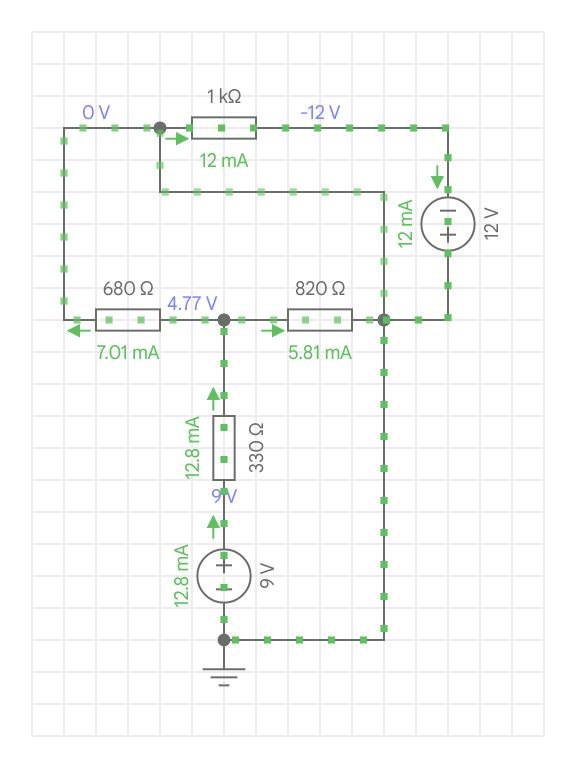
\includegraphics[width=.8\textwidth]{fig1}
	\label{fig3}
	 \caption{Simulación del circuito de la Figura 2}
\end{figure}


\end{document}